\documentclass[conference]{IEEEtran}

\usepackage{tikz}
\usetikzlibrary{chains}

\tikzset{%
  box/.style={draw,text height=1.5ex,text depth=.5ex}
}

\newcommand{\tikzFlow}[3]{%
  \begin{tikzpicture}
    \begin{scope}[start chain,every node/.style={box,on chain},node distance=2cm]
      \node (a) {Yosys};
      \node (b) {ABC};
      \node (c) {RevKit};
    \end{scope}

    \begin{scope}[every node/.style={text height=1.5ex,text depth=.5ex,inner sep=1pt,above,midway}]
      \draw[<-] (a.west) -- ++(left:1.5cm) node {verilog};
      \draw[->] (a) -- (b) node {blif};
      \draw[->] (b) -- (c) node {#1};
      \draw[->] (c.east) -- ++(right:1.5cm) node {real};
    \end{scope}

    \begin{scope}[every node/.style={align=center,anchor=north,font=\ttfamily\footnotesize}]
      \node at (a.south) {read\_verilog \\ hierarchy \\ proc; flatten \\ opt; techmap; opt \\ write\_blif};
      \node at (b.south) {#2};
      \node at (c.south) {#3};
    \end{scope}
  \end{tikzpicture}
}

\newcommand{\tikzFlowESOP}{%
  \tikzFlow{esop}
           {read\_blif \\ st; clp; sop; fx \\ st; dc2 \\ \&get \\ \&exorcism}
           {esopbs \\ write\_real}
}

\newcommand{\tikzFlowPLA}{%
  \tikzFlow{pla}
           {read\_blif \\ st \\ dc2$^5$ \\ clp \\ write\_pla}
           {read\_pla \\ embed -b \\ tbs -s \\ write\_real}
}

%%% Local Variables:
%%% mode: latex
%%% TeX-master: "notes"
%%% End:



\usepackage{listings}
\usepackage{tikz}
\usetikzlibrary{positioning,shapes,shadows,arrows}

\usepackage{microtype}
%\def\baselinestretch{.98}

% \title{Quantum Design Automation}
\title{Design Automation for Quantum Architectures}
\author{%
  \IEEEauthorblockN{Martin Roetteler \qquad Krysta M. Svore \qquad Dave Wecker \qquad Nathan Wiebe}
  \IEEEauthorblockA{%
Microsoft Research, Redmond, WA, USA
  }
}

\newcommand{\rev}[1]{{#1}}
\usepackage[bold]{hhtensor}
\usepackage{complexity}
\usepackage{amsmath, amssymb, amsthm, amsfonts, latexsym}

\usepackage[caption=false]{subfig}
    \def\subfigureautorefname{Figure}

\newcommand{\eq}[1]{Eq.~\hyperref[eq:#1]{(\ref*{eq:#1})}}
\renewcommand{\sec}[1]{\hyperref[sec:#1]{Section~\ref*{sec:#1}}}
\newcommand{\app}[1]{\hyperref[app:#1]{Appendix~\ref*{app:#1}}}
\newcommand{\apx}[1]{\hyperref[apx:#1]{Appendix~\ref*{apx:#1}}}
\newcommand{\tab}[1]{\hyperref[tab:#1]{Table~\ref*{tab:#1}}}
\newcommand{\fig}[1]{\hyperref[fig:#1]{Figure~\ref*{fig:#1}}}
\newcommand{\figa}[2]{\hyperref[fig:#1]{Figure~\ref*{fig:#1}#2}}
\newcommand{\figx}[2]{\hyperref[fig:#1]{Figure~\ref*{fig:#1}(#2)}}
\newcommand{\thm}[1]{\hyperref[thm:#1]{Theorem~\ref*{thm:#1}}}
\newcommand{\lem}[1]{\hyperref[lem:#1]{Lemma~\ref*{lem:#1}}}
\newcommand{\cor}[1]{\hyperref[cor:#1]{Corollary~\ref*{cor:#1}}}
\newcommand{\defn}[1]{\hyperref[def:#1]{Definition~\ref*{def:#1}}}
\newcommand{\alg}[1]{\hyperref[alg:#1]{Algorithm~\ref*{alg:#1}}}
\newcommand{\prob}[1]{\hyperref[prob:#1]{Problem~\ref*{prob:#1}}}
\newcommand{\openone}{1\!\!1}

\newcommand{\up}[1]{\push{\raisebox{6pt}{$#1$}}}

\newcommand{\ket}[1]{\left| #1\right\rangle}        % ket vector
\newcommand{\bra}[1]{\left\langle #1\right|}        % bra vector
\newcommand{\kets}[1]{| #1 \rangle}        % small ket vector
\newcommand{\bras}[1]{\langle #1 |}        % small bra vector
\newcommand{\braket}[2]{\langle #1 | #2 \rangle} % <x|y>
\newcommand{\ketbra}[2]{| #1 \rangle\!\langle #2 |} % <x|y>
\newcommand{\bigket}[1]{\left| #1\right\rangle}        % ket vector
\newcommand{\bigbra}[1]{\left| #1\right\rangle}        % ket vector

\usepackage[colorlinks]{hyperref}
\usepackage{url}
\usepackage{complexity}
\usepackage{hypcap}

\newcommand{\Liquid}{LIQ$Ui\ket{}$\ }

\tikzstyle{box}=[rectangle,dotted,draw=black, rounded corners, drop shadow,text centered, anchor=north, text=black, text width=2cm,scale=0.8]
\tikzstyle{styMat}=[fill=gray!40,matrix anchor=north]
\tikzstyle{styGrn}=[box,fill=green!80]
\tikzstyle{styYel}=[box,fill=yellow!80]
\tikzstyle{styAqu}=[box,fill=blue!20!yellow]
\tikzstyle{styBlu}=[box,fill=blue!40]
\tikzstyle{styRed}=[box,fill=red!40]
\tikzstyle{styOra}=[box,fill=orange!40]
\tikzstyle{myarrow}=[->,>=stealth,very  thick]


\definecolor{greencomments}{rgb}{0,0.5,0}

\lstdefinelanguage{FSharp}%
{morekeywords={let, new, match, with, rec, open, module, namespace, type, of, member, %
and, for, while, true, false, in, do, begin, fun, function, return, yield, try, %
mutable, if, then, else, cloud, async, static, use, abstract, interface, inherit, finally },
  otherkeywords={ let!, return!, do!, yield!, use!, var, from, select, where, order, by },
  keywordstyle=\color{blue},
  sensitive=true,
  basicstyle=\ttfamily,
	breaklines=true,
  xleftmargin=\parindent,
  aboveskip=\bigskipamount,
	tabsize=4,
  morecomment=[l][\color{greencomments}]{///},
  morecomment=[l][\color{greencomments}]{//},
  morecomment=[s][\color{greencomments}]{{(*}{*)}},
  morestring=[b]",
  showstringspaces=false,
  literate={`}{\`}1,
  stringstyle=\color{red},
}
\lstdefinelanguage{qc}%
{morekeywords={CNOT, CCNOT},
  otherkeywords={ let!, return!, do!, yield!, use!, var, from, select, where, order, by },
  keywordstyle=\color{red},
  sensitive=true,
  basicstyle=\ttfamily,
	breaklines=true,
  xleftmargin=\parindent,
  aboveskip=\bigskipamount,
	tabsize=4,
  morecomment=[l][\color{greencomments}]{///},
  morecomment=[l][\color{greencomments}]{//},
  morecomment=[s][\color{greencomments}]{{(*}{*)}},
  morestring=[b]",
  showstringspaces=false,
  literate={`}{\`}1,
  stringstyle=\color{red},
}

\usepackage{tabularx}
\newcommand{\REVS}{{\textsc{Revs}}}
\newcommand{\REVER}{{\textsc{ReVeR}}}
\newcommand{\LIQUID}{{LIQ{\em Ui}$|\rangle$}}
\newcommand{\mypar}[1]{{\textbf{#1.}}}
\newcommand{\nix}[1]{{}}

\newcommand{\N}{{\mathbb{N}}}

\renewcommand{\textsf}[1]{\textrm{#1}}
%syntax
\newcommand{\rlet}[3]{\textsf{let } #1 = #2 \textsf{ in } #3}
\newcommand{\rfun}[2]{\lambda #1.#2}
\newcommand{\rapply}[2]{(#1\; #2)}
\newcommand{\rseq}[2]{#1; #2}
\newcommand{\rif}[3]{\textsf{if } #1 \textsf{ then } #2 \textsf{ else } #3}
\newcommand{\rfor}[4]{\textsf{for } #1 \textsf{ in } #2..#3 \textsf{ do } #4}
\newcommand{\rassign}[2]{#1\leftarrow#2}
\newcommand{\rtrue}{\textsf{true}}
\newcommand{\rfalse}{\textsf{false}}
\newcommand{\runit}{\textsf{unit}}
\newcommand{\rxor}[2]{#1\textsf{ $<>$ }#2}
\newcommand{\rand}[2]{#1\textsf{ \&\& }#2}
\newcommand{\ror}[2]{#1\;||\;#2}
\newcommand{\rnot}[1]{\textsf{not }#1}
\newcommand{\rregister}[2]{\textsf{register } #1 \dots #2}
\newcommand{\rindex}[2]{#1.[#2]}
\newcommand{\rslice}[3]{#1.[#2..#3]}
\newcommand{\rappend}[2]{\textsf{append } #1\; #2}
\newcommand{\rrotate}[2]{\textsf{rotate } #1\; #2}
\newcommand{\rclean}[1]{\textsf{clean } #1}
\newcommand{\rassert}[1]{\textsf{assert } #1}

%    Q-circuit version 2
%    Copyright (C) 2004  Steve Flammia & Bryan Eastin
%    Last modified on: 9/16/2011
%
%    This program is free software; you can redistribute it and/or modify
%    it under the terms of the GNU General Public License as published by
%    the Free Software Foundation; either version 2 of the License, or
%    (at your option) any later version.
%
%    This program is distributed in the hope that it will be useful,
%    but WITHOUT ANY WARRANTY; without even the implied warranty of
%    MERCHANTABILITY or FITNESS FOR A PARTICULAR PURPOSE.  See the
%    GNU General Public License for more details.
%
%    You should have received a copy of the GNU General Public License
%    along with this program; if not, write to the Free Software
%    Foundation, Inc., 59 Temple Place, Suite 330, Boston, MA  02111-1307  USA

% Thanks to the Xy-pic guys, Kristoffer H Rose, Ross Moore, and Daniel Müllner,
% for their help in making Qcircuit work with Xy-pic version 3.8.  
% Thanks also to Dave Clader, Andrew Childs, Rafael Possignolo, Tyson Williams,
% Sergio Boixo, Cris Moore, Jonas Anderson, and Stephan Mertens for helping us test 
% and/or develop the new version.

\usepackage[color]{xy}
\UseCrayolaColors
\xyoption{matrix}
\xyoption{frame}
\xyoption{arrow}
\xyoption{arc}

\usepackage{ifpdf}
\ifpdf
\else
\PackageWarningNoLine{Qcircuit}{Qcircuit is loading in Postscript mode.  The Xy-pic options ps and dvips will be loaded.  If you wish to use other Postscript drivers for Xy-pic, you must modify the code in Qcircuit.tex}
%    The following options load the drivers most commonly required to
%    get proper Postscript output from Xy-pic.  Should these fail to work,
%    try replacing the following two lines with some of the other options
%    given in the Xy-pic reference manual.
\xyoption{ps}
\xyoption{dvips}
\fi

% The following resets Xy-pic matrix alignment to the pre-3.8 default, as
% required by Qcircuit.
\entrymodifiers={!C\entrybox}

%\newcommand{\bra}[1]{{\left\langle{#1}\right\vert}}
%\newcommand{\ket}[1]{{\left\vert{#1}\right\rangle}}
    % Defines Dirac notation. %7/5/07 added extra braces so that the commands will work in subscripts.
\newcommand{\qw}[1][-1]{\ar @{-} [0,#1]}
\newcommand{\eqw}[1][-1]{\ar @{-} @[Red] [0,#1]}
    % Defines a wire that connects horizontally.  By default it connects to the object on the left of the current object.
    % WARNING: Wire commands must appear after the gate in any given entry.
\newcommand{\qwx}[1][-1]{\ar @{-} [#1,0]}
    % Defines a wire that connects vertically.  By default it connects to the object above the current object.
    % WARNING: Wire commands must appear after the gate in any given entry.
\newcommand{\cw}[1][-1]{\ar @{=} [0,#1]}
    % Defines a classical wire that connects horizontally.  By default it connects to the object on the left of the current object.
    % WARNING: Wire commands must appear after the gate in any given entry.
\newcommand{\cwx}[1][-1]{\ar @{=} [#1,0]}
    % Defines a classical wire that connects vertically.  By default it connects to the object above the current object.
    % WARNING: Wire commands must appear after the gate in any given entry.
\newcommand{\gate}[1]{*+<.6em>{#1} \POS ="i","i"+UR;"i"+UL **\dir{-};"i"+DL **\dir{-};"i"+DR **\dir{-};"i"+UR **\dir{-},"i" \qw}
\newcommand{\eboxgate} [1]{*+<.6em>{#1} \POS ="i","i"+UR;"i"+UL **[red]\dir{-};"i"+DL **[red]\dir{-};"i"+DR **[red]\dir{-};"i"+UR **[red]\dir{-},"i" \eqw}
\newcommand{\circgate}[1]{*+<0.6em>[o][F-]{#1} \eqw}
\newcommand{\ecircgate}[1]{*+<0.6em>[o][F-:red]{#1} \eqw}
\newcommand{\filtergt}[1]{\eboxgate{\scriptscriptstyle{#1}}}
\newcommand{\idealdec}{*+<1.2em>{\phantom{*}} \POS ="i","i"+UL;"i"+DL **[red]\dir{-};"i"+R **[red]\dir{-};"i"+UL **[red]\dir{-},"i" \eqw}

    % Boxes the argument, making a gate.
\newcommand{\meter}{*=<1.8em,1.4em>{\xy ="j","j"-<.778em,.322em>;{"j"+<.778em,-.322em> \ellipse ur,_{}},"j"-<0em,.4em>;p+<.5em,.9em> **\dir{-},"j"+<2.2em,2.2em>*{},"j"-<2.2em,2.2em>*{} \endxy} \POS ="i","i"+UR;"i"+UL **\dir{-};"i"+DL **\dir{-};"i"+DR **\dir{-};"i"+UR **\dir{-},"i" \qw}
    % Inserts a measurement meter.
    % In case you're wondering, the constants .778em and .322em specify
    % one quarter of a circle with radius 1.1em.
    % The points added at + and - <2.2em,2.2em> are there to strech the
    % canvas, ensuring that the size is unaffected by erratic spacing issues
    % with the arc.
\newcommand{\measure}[1]{*+[F-:<.9em>]{#1} \qw}
    % Inserts a measurement bubble with user defined text.
\newcommand{\measuretab}[1]{*{\xy*+<.6em>{#1}="e";"e"+UL;"e"+UR **\dir{-};"e"+DR **\dir{-};"e"+DL **\dir{-};"e"+LC-<.5em,0em> **\dir{-};"e"+UL **\dir{-} \endxy} \qw}
    % Inserts a measurement tab with user defined text.
\newcommand{\measureD}[1]{*{\xy*+=<0em,.1em>{#1}="e";"e"+UR+<0em,.25em>;"e"+UL+<-.5em,.25em> **\dir{-};"e"+DL+<-.5em,-.25em> **\dir{-};"e"+DR+<0em,-.25em> **\dir{-};{"e"+UR+<0em,.25em>\ellipse^{}};"e"+C:,+(0,1)*{} \endxy} \qw}
\newcommand{\emeasureD}[1]{*{\xy*+=<0em,.1em>{#1}="e";"e"+UR+<0em,.25em>;"e"+UL+<-.5em,.25em> **[red]\dir{-};"e"+DL+<-.5em,-.25em> **[red]\dir{-};"e"+DR+<0em,-.25em> **[red]\dir{-};{"e"+UR+<0em,.25em>\ellipse{}};"e"+C:,+(0,1)*{} \endxy} \qw}
    % Inserts a D-shaped measurement gate with user defined text.
\newcommand{\multimeasure}[2]{*+<1em,.9em>{\hphantom{#2}} \qw \POS[0,0].[#1,0];p !C *{#2},p \drop\frm<.9em>{-}}
    % Draws a multiple qubit measurement bubble starting at the current position and spanning #1 additional gates below.
    % #2 gives the label for the gate.
    % You must use an argument of the same width as #2 in \ghost for the wires to connect properly on the lower lines.
\newcommand{\multimeasureD}[2]{*+<1em,.9em>{\hphantom{#2}} \POS [0,0]="i",[0,0].[#1,0]="e",!C *{#2},"e"+UR-<.8em,0em>;"e"+UL **\dir{-};"e"+DL **\dir{-};"e"+DR+<-.8em,0em> **\dir{-};{"e"+DR+<0em,.8em>\ellipse^{}};"e"+UR+<0em,-.8em> **\dir{-};{"e"+UR-<.8em,0em>\ellipse^{}},"i" \qw}
    % Draws a multiple qubit D-shaped measurement gate starting at the current position and spanning #1 additional gates below.
    % #2 gives the label for the gate.
    % You must use an argument of the same width as #2 in \ghost for the wires to connect properly on the lower lines.
\newcommand{\control}{*!<0em,.025em>-=-<.2em>{\bullet}}
    % Inserts an unconnected control.
\newcommand{\controlo}{*+<.01em>{\xy -<.095em>*\xycircle<.19em>{} \endxy}}
    % Inserts a unconnected control-on-0.
\newcommand{\ctrl}[1]{\control \qwx[#1] \qw}
    % Inserts a control and connects it to the object #1 wires below.
\newcommand{\ctrlo}[1]{\controlo \qwx[#1] \qw}
    % Inserts a control-on-0 and connects it to the object #1 wires below.
\newcommand{\targ}{*+<.02em,.02em>{\xy ="i","i"-<.39em,0em>;"i"+<.39em,0em> **\dir{-}, "i"-<0em,.39em>;"i"+<0em,.39em> **\dir{-},"i"*\xycircle<.4em>{} \endxy} \qw}
    % Inserts a CNOT target.
\newcommand{\qswap}{*=<0em>{\times} \qw}
    % Inserts half a swap gate.
    % Must be connected to the other swap with \qwx.
\newcommand{\multigate}[2]{*+<1em,.9em>{\hphantom{#2}} \POS [0,0]="i",[0,0].[#1,0]="e",!C *{#2},"e"+UR;"e"+UL **\dir{-};"e"+DL **\dir{-};"e"+DR **\dir{-};"e"+UR **\dir{-},"i" \qw}
    % Draws a multiple qubit gate starting at the current position and spanning #1 additional gates below.
    % #2 gives the label for the gate.
    % You must use an argument of the same width as #2 in \ghost for the wires to connect properly on the lower lines.
\newcommand{\ghost}[1]{*+<1em,.9em>{\hphantom{#1}} \qw}
    % Leaves space for \multigate on wires other than the one on which \multigate appears.  Without this command wires will cross your gate.
    % #1 should match the second argument in the corresponding \multigate.
\newcommand{\push}[1]{*{#1}}
    % Inserts #1, overriding the default that causes entries to have zero size.  This command takes the place of a gate.
    % Like a gate, it must precede any wire commands.
    % \push is useful for forcing columns apart.
    % NOTE: It might be useful to know that a gate is about 1.3 times the height of its contents.  I.e. \gate{M} is 1.3em tall.
    % WARNING: \push must appear before any wire commands and may not appear in an entry with a gate or label.
\newcommand{\gategroup}[6]{\POS"#1,#2"."#3,#2"."#1,#4"."#3,#4"!C*+<#5>\frm{#6}}
    % Constructs a box or bracket enclosing the square block spanning rows #1-#3 and columns=#2-#4.
    % The block is given a margin #5/2, so #5 should be a valid length.
    % #6 can take the following arguments -- or . or _\} or ^\} or \{ or \} or _) or ^) or ( or ) where the first two options yield dashed and
    % dotted boxes respectively, and the last eight options yield bottom, top, left, and right braces of the curly or normal variety.  See the Xy-pic reference manual for more options.
    % \gategroup can appear at the end of any gate entry, but it's good form to pick either the last entry or one of the corner gates.
    % BUG: \gategroup uses the four corner gates to determine the size of the bounding box.  Other gates may stick out of that box.  See \prop.

\newcommand{\rstick}[1]{*!L!<-.5em,0em>=<0em>{#1}}
    % Centers the left side of #1 in the cell.  Intended for lining up wire labels.  Note that non-gates have default size zero.
\newcommand{\lstick}[1]{*!R!<.5em,0em>=<0em>{#1}}
    % Centers the right side of #1 in the cell.  Intended for lining up wire labels.  Note that non-gates have default size zero.
\newcommand{\ustick}[1]{*!D!<0em,-.5em>=<0em>{#1}}
    % Centers the bottom of #1 in the cell.  Intended for lining up wire labels.  Note that non-gates have default size zero.
\newcommand{\dstick}[1]{*!U!<0em,.5em>=<0em>{#1}}
    % Centers the top of #1 in the cell.  Intended for lining up wire labels.  Note that non-gates have default size zero.
\newcommand{\Qcircuit}{\xymatrix @*=<0em>}
    % Defines \Qcircuit as an \xymatrix with entries of default size 0em.
\newcommand{\link}[2]{\ar @{-} [#1,#2]}
    % Draws a wire or connecting line to the element #1 rows down and #2 columns forward.
\newcommand{\pureghost}[1]{*+<1em,.9em>{\hphantom{#1}}}
    % Same as \ghost except it omits the wire leading to the left. 
%%%%%%%%%%%%%%%%%%%%%%%%%%%%%%%%%%%%%%%%%%%%%%%%%%%%%%%%%%%%%%%%%%%%%%%%%%%%%%%%%%%%%%%%%%
\newcommand{\multiprepareC}[2]{*+<1em,.9em>{\hphantom{#2}}\save[0,0].[#1,0];p\save !C
  *{#2},p+RU+<0em,0em>;+LU+<+.8em,0em> **\dir{-}\restore\save +RD;+RU **\dir{-}\restore\save
  +RD;+LD+<.8em,0em> **\dir{-} \restore\save +LD+<0em,.8em>;+LU-<0em,.8em> **\dir{-} \restore \POS
  !UL*!UL{\cir<.9em>{u_r}};!DL*!DL{\cir<.9em>{l_u}}\restore}
   % Draws a multiple qubit reverse-D-shaped preparation gate starting at the current position and spanning #1 additional gates below.
   % #2 gives the label for the gate.
   % You must use an argument of the same width as #2 in \pureghost for the wires to connect properly on
% the lower lines.
\newcommand{\prepareC}[1]{*{\xy*+=+<.5em>{\vphantom{#1\rule{0em}{.1em}}}*\cir{l^r};p\save*!L{#1} \restore\save+UC;+UC+<.5em,0em>*!L{\hphantom{#1}}+R **\dir{-} \restore\save+DC;+DC+<.5em,0em>*!L{\hphantom{#1}}+R **\dir{-} \restore\POS+UC+<.5em,0em>*!L{\hphantom{#1}}+R;+DC+<.5em,0em>*!L{\hphantom{#1}}+R **\dir{-} \endxy}}
   % Inserts a reverse-D-shaped preparation gate with user defined text.
\newcommand{\poloFantasmaCn}[1]{{{}^{#1}_{\phantom{#1}}}}


\usetikzlibrary{calc}

\begin{document}

\maketitle

\begin{abstract}
We survey recent strides made towards building a software framework that is capable of compiling quantum algorithms from a high-level algorithm description down to physical gates that can be implemented on a fault-tolerant quantum computer. We discuss why compilation and design automation tools such as the ones in our framework are key for tackling the grand challenge of building a scalable quantum computer. We then describe specialized libraries that have been developed using the \Liquid programming language. This includes reversible circuits for arithmetic as well as new, truly quantum approaches that rely on quantum computer architectures that allow the probabilistic execution of gates, a model that can reduce time and space overheads in some cases. We highlight why these libraries are useful for the implementation of many quantum algorithms. Finally, we survey the tool \REVS~that facilitate resource efficient compilation of higher-level irreversible programs into lower-level reversible circuits while trying to optimize the memory footprint of the resulting reversible networks. This is motivated by the limited availability of qubits for the foreseeable future. 
\end{abstract}

\section{Introduction}
Quantum computing has begun to take off over the last few years. In part, this is thanks to dramatic improvements in hardware and continued improvements in quantum algorithms.  Now the technology
is perched at the threshold of offering meaningful speedups for problems that are both scientifically and industrially relevant~\cite{barends2014superconducting,cross2015quantum,o2016scalable,benedetti2016estimation}.  

On the other hand, as we push past this first generation of quantum devices, a host of problems emerge for those who wish to develop software for large scale quantum computers.  Even basic questions, such as ``how do we program quantum computers?'' do not have easy answers.  Furthermore, some of our most important quantum algorithms such as linear-systems algorithms and certain classes of quantum simulation algorithms require reversible analogues of arithmetic and elementary functions~\cite{harrow2009quantum,babbush2015exponentially,kivlichan2016bounding}. Existing quantum circuits for arithmetic require a prohibitive number of quantum bits (qubits) and cannot be automatically generated~\cite{BHP+15}.  Even if such hand crafted networks are provided then verifying and validating them remains a major challenge.  These problems need to be solved to realize the promise of quantum computing.

In this survey, we highlight some of the ongoing work towards solving these problems before they prove to be a stumbling block for quantum computing. Researchers at Microsoft Research developed a quantum programming language \Liquid~\cite{WS:2014} that enables programmers to translate high-level ideas into concrete quantum circuits and test the resulting networks. In another development, a language called \REVS~was developed that can compile irreversible classical code into reversible networks---e.g., over the Toffoli gate set---in a way that is cognizant of space and time tradeoffs~\cite{PRS15}. 

Reversible networks have the oft under-appreciated feature that they can be tested efficiently for faults that might be present in a physical implementation, say, on an actual quantum computer~\cite{HRS16}. The intended execution can always be predicted, at a fine level of granularity that goes beyond mere end-to-end target functionality.  Specifically, we can predict it by partially running the reversible network for a certain number of steps on an input that corresponds to a classical input, i.e., a computational basis state. This might be one advantage that the design of quantum libraries as reversible networks offers over other approaches, e.g., genuine quantum approaches where the identification of faults can be significantly more challenging due to the fact that the computational state is in a superposition, e.g., extended across many basis states, even when the computer is in a debugging mode and probes only basis states. 

Another advantage of reversible design is that formal verification techniques can be applied to the problem of ascertaining the correctness of either a given network or a compiler implementation. The former falls in the domain of equivalence checking for circuits, a topic that has been addressed e.g. in \cite{VMH:2007}. See also \cite{SRWD:2017} for a recent example where correctness of generated circuits was checked by means of BDD based checkers.  The latter correctness, falls in the domain of compiler verification where the transformation of the compiler are mathematically proven to be correct, typically with the help of an automatic proof checker. \REVER~\cite{ARS16}, which can be thought of as a restricted version of the \REVS~compiler, was proven to be correct along these lines by using the proof checker F*.  This guarantees that a) any Toffoli network that is generated from an F\# functional description by \REVER~actually matches this functional description as the function computed on the output wires of the network, and b) any clean ancillas that might be needed during the computation are provably returned back into a clean state. Unlike classical computing, ancillas need to be reverted to remove quantum entanglement in quantum computing.

These ideas are then used in a new approach to function synthesis that leverages the decades of progress in irreversible circuit synthesis to automatically generate highly efficient circuits for arithmetic and standard scientific functions that are even more efficient than the best hand-crafted solutions that currently exist.  Finally, we discuss new quantum approaches for arithmetic and function synthesis that do not require compilation into classical reversible circuits as an intermediate step~\cite{WR16}.  This reveals that even for well understood tasks like arithmetic, quantum computing can provide new ways of thinking about processing data that have no classical analogue. 

\section{Quantum programming in \Liquid} %Liquid

There is no shortage of quantum programming languages. The list includes imperative, C-like languages QCL \cite{Oemer:2005}, QLanguage \cite{BCS:2003}, and Scafford/ScaffCC~\cite{HPJ+:2015,KPK+:2015}, functional languages embedded in Haskell such as Quipper~~\cite{GLR+:2013a,GLR+:2013b}, the Quantum I/O Monad~\cite{AG:2009} and QuaFL/QuiGL~\cite{LST+:2013,LR:2013}. Also, there are several languages for reversible computing based on Janus and various extensions~\cite{YG:2007,Thomsen:2012,Perumalla:2014}. 
Furthermore, there are toolkits such as CirKit/RevKit~\cite{SFWD12} that can assist lower-level functional synthesis from logic descriptions and when put together with a tool flow that can compile from a hardware description language such as Verilog into netlists, can provide high-level to Toffoli gate level compilation. 

In the following we describe the approach underlying \LIQUID~\cite{WS:2014}, which is a functional quantum programming language embedded in the .NET host language F\# and developed at Microsoft Research. \LIQUID~is fundamentally a circuit description language for quantum circuits, however, it also provides support for higher level programming that ultimately will help a programmer to develop quantum computational thinking that is not necessarily centered around circuits but rather on the mathematical functions that are the abstractions of concrete embodiments given by circuits. 

In contrast to many of the mentioned approaches, \Liquid was designed and architected explicitly with quantum hardware in mind. 
For instance, one of the underlying design assumptions is that qubits are real entities, have lifetimes and are fundamentally mutable objects, which led to the choice of our basic qubit type.
Also, while other languages also come equipped with simulators, the \Liquid simulators are highly optimized, taking advantage of many available techniques, including custom memory management, cache coherence analysis, parallelization, ``gate growing", and virtualization (running in the cloud). The \Liquid simulation environment allows thorough investigation of quantum algorithms under noise, physical device constraints, and simulation.


\begin{figure}[t]
\centering
\begin{tikzpicture}[node distance=0.1cm]]

\matrix(matLang)[styMat,every node/.style={styGrn}] {
\node[very thick,solid] {\textbf{Language:}}; & \node {F\#}; &
\node {Script}; & \node{C\#};  \\
} ;
\matrix(matGate)[styMat,below =0.2 of matLang,every node/.style={styYel}] {
\node[very thick,solid] {\textbf{Functions:}}; & \node {Gates}; & \node{Libraries}; & \node[very thick,dashed]{REVS}; \\
} ;

\matrix(matCirc)[styMat,below =0.2 of matGate,every node/.style={styRed}] {
\node[very thick,solid] {\textbf{Circuits:}}; & \node {Optimize}; & \node {QECC}; & \node {Replace}; \\
 & \node{Resource}; & \node{Export}; & \node{Render...}; \\
} ;

\matrix(matSim)[styMat, below = 0.2 of matCirc,every node/.style={styAqu}] {
\node[very thick,solid] {\textbf{Simulators:}}; & \node {Universal}; & \node {Hamiltonian}; & \node {Stabilizer};  \\
& \node{Toffoli};  \\
} ;

\matrix(matRun)[styMat, below =0.2 of matSim,every node/.style={styBlu}] {
\node[very thick,solid] {\textbf{Runtimes:}}; & \node {Client}; &
\node {Service}; & \node {Cloud}; \\
} ;

\matrix(matExp)[styMat, below =0.2 of matRun,every node/.style={styOra}] {
\node[very thick,solid] {\textbf{Backends:}}; & \node {Classical}; &
& \node {Quantum}; & & \\
} ;

\draw[myarrow] (matLang.south) -- (matGate.north);
\draw[myarrow] (matGate.south) -- (matCirc.north);
\draw[myarrow] (matCirc.south) -- (matSim.north);
\draw[myarrow] (matSim.south) -- (matRun.north);
\draw[myarrow] (matGate.west) -- ++(-0.5	,0) |- (matSim.west);
\draw[myarrow] (matCirc.east) -- ++(0.5,0) |- (matExp.east);

\end{tikzpicture}
\caption{\label{fig:arch}\Liquid architecture overview. Shown are two natural flows, namely the passing of functions to a classical simulator and the passing of emitted circuits to a hardware backend for execution. }
\end{figure}

\subsection{Software architecture}

A general overview of the \LIQUID~software architecture is shown in \fig{arch}. While for a more detailed breakdown of the stages we refer to \cite{WS:2014}, here we provide a brief description of the main features and interplay between stages and highlight  particular aspects that are germane to each stage. 

\noindent $\bullet$ {\em Language}: The embedding into F\# was chosen primarily due to .NET support, object-oriented and functional programming, ease of using reflection and pattern matching which helps with walking complex datastructures, plus a wealth of external libraries. Additions introduced by \Liquid to the host language include types {\sc Qubit}, {\sc Ket}, {\sc Gate}, {\sc Operation}, and {\sc Circuit}. Notably, besides von Neumann measurements, \Liquid also supports also POVMs as a basic gate type. 

\noindent $\bullet$ {\em Functions}: The most basic, but at the same time: most important, example of a function is the one of an executable gate. All \Liquid gates are user defined functions or class instances that can be extended by the user in many ways. Note that while it is possible to apply introspection to a function (such as asking e.g. whether it corresponds to a unitary operator), it is not mapped to a circuit yet. This allows the freedom to allow many different possible abstract interpretations for any given \Liquid function. %: one can simulate it on several different runtimes, one can render it into many different graphical representations, one can transform it into a circuit which then itself can be turned into different futher representations, i.e., quantum instructions can be emitted that can be executed by actual quantum computer hardware. Also, examples of functions arise in generator libraries which are executable programs that produce functions open instantiation with given parameter values. For example, signal processing transforms such as discrete Fourier, sine, cosine, and wavelet transforms of a given length, or arithmetic operations of given bitsize. 
The \REVS~compiler, shown as dashed box in \fig{arch} can compile  classical, irreversible code into \Liquid functions that can then be further processed. 

\noindent $\bullet$ {\em Circuits}: This level deals with the data structures that most researchers in quantum computing are familiar with: circuits that are composed over an elementary gate set and operate on a certain number of qubits. Many ways to manipulate circuits are possible, including a) further decomposition into lower level gates, b) peep-hole style optimization via rewriting, c) optimizations for trading off size and width, d) resource estimation, e) wrapping with fault-tolerance methods. 


\noindent $\bullet$ {\em Simulators}: Simulators that are currently supported include a) a universal simulator that essentially performs the matrix-vector product for a given initial state vector and given unitary corresponding to a circuit. %, however, many optimizations are implemented to speed things up. %This includes classes that prevent unnecessary allocation and re-allocation and garbage collection, classes that ensure extremely stable memory footprint during simulation, in some cases even for hundreds of millions of gates, enhanced parallelization and memory management, e.g., via reordering data to keep it cache local. 
There are various special purpose simulators such as b) a simulator for Clifford circuits based on tracking stabilizer tableaux. Also, there are c) simulators for Hamiltonians, which is particularly useful for applications in quantum chemistry, and d) simulators for reversible circuits, such as Toffoli circuits which is based on tracking basis states as they propagate through the network. 

\noindent $\bullet$ {\em Runtimes}: Currently, for development, \Liquid supports compilation in environments such as Visual Studio under Windows, as well as full compatibility under Linux/Mono and Mac OS. \Liquid is available on {\it github.com/StationQ/Liquid}. Runtimes supported are client/server versions, as well as an Azure based cloud service. There are several ways in which \Liquid code can be executed, e.g., from the command line running the .NET Common Language Runtime, or directly in a Visual Studio interactive session (particularly useful for script files), or in a normal Visual Studio development mode.


\noindent $\bullet$ {\em Backends}: Besides the backend of a classical computer system, many possible quantum computer embodiments can in principle be latched onto via \Liquid\!\!. 

\subsection{Hardware design space}

Depending on the experimental device design, a quantum computer architecture may allow arbitrary long-range interactions between any two physical qubits or may restrict interactions to occur on spatially neighboring qubits. The former model is represented by a complete graph with an edge between every pair of nodes while the latter model could be represented, for example, by a two-dimensional regular grid. In both cases, we assume concurrent application of gates. 
Concatenated codes readily support the former abstract concurrent architecture, and may also be designed to support a nearest-neighbor architecture.  However, topological codes more naturally support nearest-neighbor restrictions.
The surface code tile shown in \fig{architecture}(a) represents one logical qubit encoded in 13 data qubits, with 12 syndrome qubits for error extraction.  Data qubits are represented by light nodes and syndrome qubits used to detect errors by dark nodes.  Each data qubit may interact with its four neighboring syndrome qubits.  In a complete architecture, each logical qubit is encoded in such a tile as shown in \fig{architecture}(b); to enact a two-qubit logical gate, a tile interacts with a neighboring tile through, i.e., lattice surgery \cite{HFD+:2012}.

Tiles can also be enlarged to encode several logical qubits, e.g., by introducing so-called defects \cite{Fowl12f} or displacements \cite{HG:2015}. In this case, arbitrary interactions between the qubits within a tile are possible, see e.g. \cite{HFD+:2012,PF:2015,LB:2015}. 
Considering an intermediate representation to address unitary operations at the level of braids, it is possible to perform two-qubit Clifford operations in a non-local way by braiding in space--time logical qubits that are far away; see \cite{PF:2013} for an algorithm that achieves compaction of braids. Here we assume that operations between tiles are brokered via distributed CNOT gates, similar to architectures proposed in \cite{MFC:2011,vMNM+:2006,vMeter:2014,LB:2015}. 

\begin{figure}[htb]
\centering
%\raisebox{0.2ex}{\includegraphics[scale=0.3]{}}
%\; \raisebox{5ex}{\hspace{1.4mm}$=$} \;\;
\begin{tabular}{c@{\qquad}c}
\raisebox{1ex}{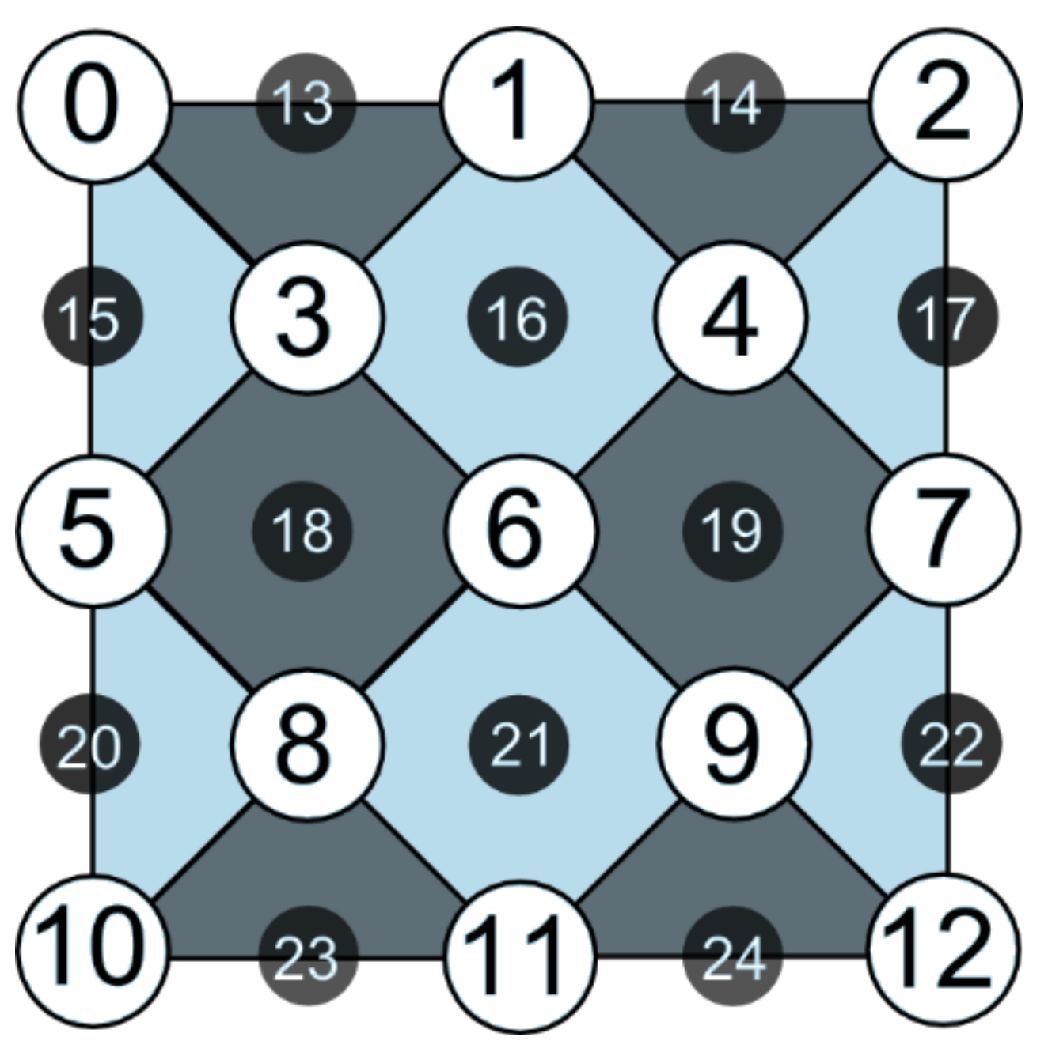
\includegraphics[height=2.8cm]{pictures/surface25_1.pdf}} &
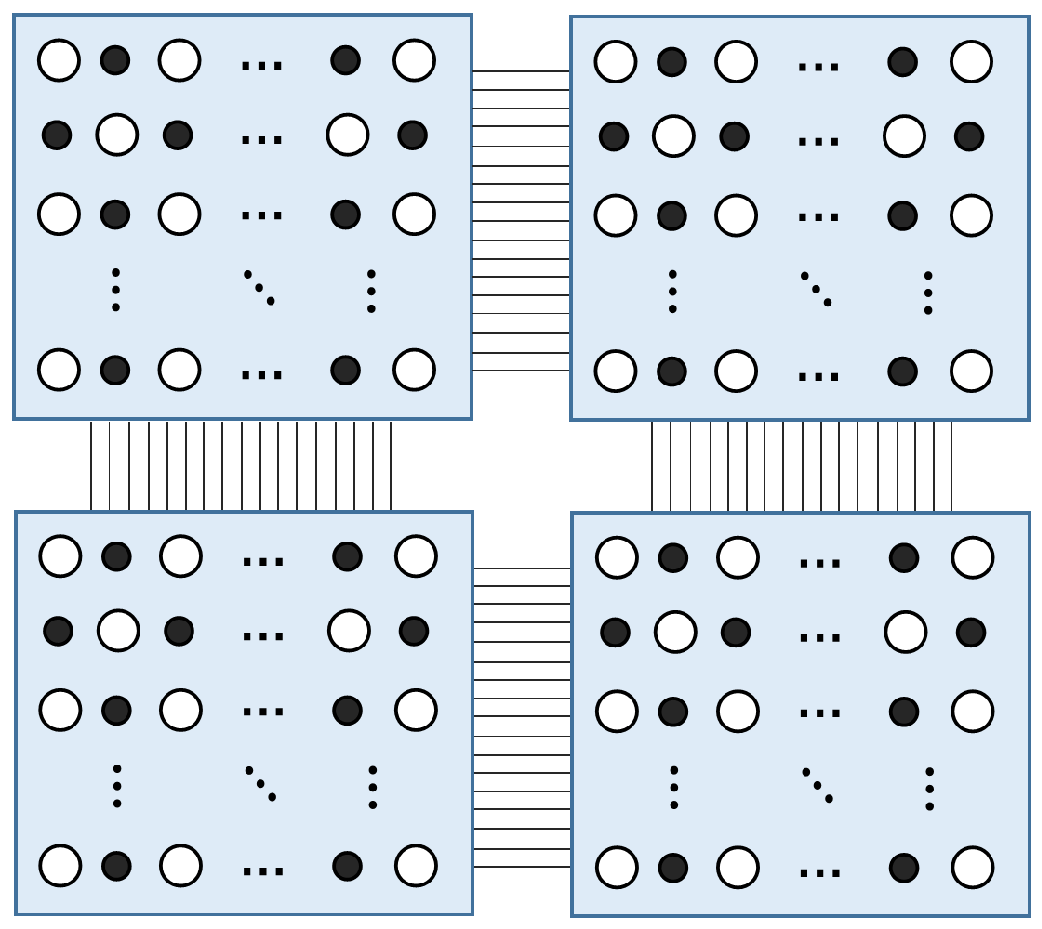
\includegraphics[height=3cm]{pictures/tiles2.pdf}\\
(a) & (b) 
\end{tabular}
\medskip
\caption{\label{fig:architecture} Surface code quantum architecture: (a) a single qubit tile with data qubits (white) and syndrome qubits (black), shown for the distance-three Surface-25 tile encoding one logical qubit \cite{TS:2014}; (b) the overall fault-tolerant architecture assumed in this paper arises from grouping several $n\times n$ surface code tiles, each one holding several logical qubits in a connected network where interactions between neighboring tiles are brokered by CNOTs.} 
\end{figure}

As far as reversible computations are concerned, the number of Toffoli gates used in the implementation of a given permutation is a basic measure of complexity. This measures the circuit {\em size} as one of the basic metrics we are interested in. Counting Toffolis only is justified from the theory of fault-tolerant quantum computing \cite{NC:2000} since the Toffoli gate (and the $T$ gate) has a substantial cost, whereas the cost of so-called Clifford gates, such as CNOT and NOT, can usually be neglected. Another related metric is the overall depth of the circuit, measured usually in the form of $T$-gate-depth. Implementations of the Toffoli gate over the Clifford$+T$ gate set are known, see e.g. \cite{Amy:2013} for realizing a Toffoli gate in $T$-depth $3$. The other basic parameter in our design space is the circuit {\em width}, measured as the maximum number of qubits needed during any point of a quantum circuit, i.e., the maximum number of input qubits, output qubits, and ancilla qubits. Generally, our goal is to trade time for space, i.e., to achieve a reduction in the total number of qubits required.  In turn, we are willing to pay a price in terms of a slight increase in the total number of Toffoli gates and in terms of compilation time. Our 
trade-off is justified by the limited number of qubits available in experimental quantum devices.


\section{Reversible programming in \REVS} 

\REVS~is an embedded language into the .NET language F\# and as such inherits some functions and libraries from its host language. Also, the look-and-feel of a typical \REVS~program is very similar to that of F\# programs. 
\nix{The abstract syntax of \REVS~is as follows: 
\begin{flalign*}
%	{\bf Var} \;&x & \\
%	{\bf Nat} \;&i, j\in\N & \\
%	{\bf Loc} \;&l\in\N \\
	{\bf Var} \;&x \quad {\bf Nat} \;i, j\in\N \quad \;{\bf Loc} \;l\in\N \\
	{\bf Val} \;&v ::= \runit \| l \| \rregister{l_1}{l_n} \| \rfun{x}{t} & \\
		{\bf Term} \; &t ::= \rlet{x}{t_1}{t_2} \| \rfun{x}{t} \| \rapply{t_1}{t_2} \| \rseq{t_1}{t_2} \| x \| \rassign{t_1}{t_2}& \\
			%&\hspace{1.4em}|\; \rapply{t_1}{t_2} \| \rseq{t_1}{t_2} \| %\rif{t_1}{t_2}{t_3} & \\ %\| \rfor{x}{i}{j}{t}  & \\
			&\hspace{0.0em}|\; \rtrue \| \rfalse \| \rxor{t_1}{t_2} \|  \rand{t_1}{t_2} \| \rclean{t} \| \rassert{t} & \\ % \| t_1 = t_2 \| \neg t  & \\
			&\hspace{0.0em}|\; \rregister{t_1}{t_n}\! \| \rindex{t}{i} \| \rslice{t}{i}{j} \| \rappend{t_1\!}{t_2}\! \| \rrotate{i}{t} &
		%\vspace{1em}
		%{\bf Bexp}\;\; &b ::= true \| false\| x^i \| \neg b \| b_1 \land b_2 \| b_1 \oplus b_2 \\
\end{flalign*}

 Shown is a grammar, i.e., a set of production rules. Variables are denoted by {\bf Var}, values by {\bf Val}, and terms by {\bf Term}.}

 The current implementation of the \REVS~compiler supports Booleans as basic types only. The core of the language is a simple imperative language over Boolean and array (register) types. The language is further extended with ML-style functional features, namely first-class functions and \emph{let} definitions, and a reversible domain-specific construct \emph{clean}. It should be noted also that \REVS~was designed to facilitate interoperability with the quantum programming language \LIQUID{}.
An example \REVS~program is shown in \fig{rippleCode}(a). This example implements a simple carry ripple adder of two $n$-bit integers. Shown in (b) is one of the possible target intermediate representations, namely \LIQUID{} code. 


\begin{figure*}[hbt]
\small 
\begin{tabular}{c@{\qquad\;\;\qquad}c}
\begin{lstlisting}[language=FSharp]
let rippleAdder (a:bool []) (b:bool []) =
   let n = Array.length a
   let result =  Array.zeroCreate (n)
   result.[0] <- a.[0] <> b.[0]
   let mutable carry = a.[0] && b.[0]
   result.[1] <- a.[1] <> b.[1] <> carry
   for i in 2 .. n - 1 do
      // compute outgoing carry 
      carry <- (a.[i-1] 
               && (carry <> b.[i-1])) 
               <> (carry && b.[i-1])
      result.[i]  <-  a.[i] <> b.[i] 
                      <> carry
   result
\end{lstlisting}
& 
{\small
\begin{lstlisting}[language=qc]
CNOT [ qs.[0]; qs.[10] ]
CNOT [ qs.[5]; qs.[10] ]
CCNOT [ qs.[0]; qs.[5]; qs.[15] ]
CNOT [ qs.[15]; qs.[11] ]
CNOT [ qs.[1]; qs.[11] ]
CNOT [ qs.[6]; qs.[11] ]
CNOT [ qs.[15]; qs.[17] ]
CNOT [ qs.[6]; qs.[17] ]
CCNOT [ qs.[1]; qs.[17]; qs.[16] ]
CCNOT [ qs.[15]; qs.[6]; qs.[16] ]
CNOT [ qs[6]; qs.[17] ]
CNOT [ qs.[15]; qs.[17] ]
CNOT [ qs.[16]; qs.[12] ]
...
\end{lstlisting}}
\\
(a) \REVS~source program & (b) Segment of the compiled \LIQUID~program 
\end{tabular}
\medskip
\caption{\label{fig:rippleCode} F$\#$ program that implements a carry ripple adder using a simple for loop while maintaining a running carry.}
\end{figure*}




\begin{table}[hbt]
\centering
  \begin{tabular}{crrrrcc}%r@{\!}r@{\!}r@{\!}r@{\!}r@{\!}c@{\!}r}
    \hline
    & \multicolumn{2}{c} {Eager}    &  \multicolumn{2}{c} {Bennett} &  \\
%\hline
    Name           & Bits          &   Gates       &      Bits     &       Gates  & Red.($\%$) & Time   \\
\hline\\
%    CM150           &       42      &       1696    &       71      &       1017    &  40.85      & 0.009 \\
%    CM151           &       25      &       795     &       36      &       485     &  30.56      & 0.003 \\
%    CM163           &       36      &       843     &       66      &       825     & 45.45       & 0.007\\
    DES             &       992     &       85351   &       2123    &       62425   &  53.27      & 1.720 \\
    alu4cl         &       175     &       13487   &       441     &       8867    &  60.32       & 0.101 \\ %
    apex7           &       111     &       3299    &       242     &       3077    &   54.13     & 0.031 \\ %
    b9              &       127     &       4444    &       316     &       3185    &  59.81      & 0.035 \\ %
    c8              &       80      &       4791    &       213     &       4149    &   62.44     & 0.022 \\
%    cht             &       89      &       2664    &       179     &       3025    &  50.28      & 0.019 \\
%    cmb             &       37      &       1042    &       60      &       707     &  38.33      & 0.008 \\
    comp            &       97      &       2606    &       162     &       1991    &  40.12      & 0.017 \\
    cordic          &       130     &       3094    &       262     &       2363    &  50.38      & 0.037 \\ %
    count           &       71      &       1304    &       124     &       1435    &  42.74      & 0.014 \\ %
    cu              &       36      &       1395    &       80      &       1045    &  55.00         & 0.009 \\
    dalu            &       1056    &       77482   &       3444    &       49463   &  69.34      & 1.440 \\
    decod           &       27      &       188     &       28      &       365     &  3.57       & 0.003 \\
 %   f51m            &       49      &       4684    &       69      &       2427    & 28.99       & 0.059 \\
    frg2            &       531     &       44820   &       2080    &       34117   & 74.47       & 0.472 \\
   % i10             &       1633    &       24505   &       3385    &       23489   & 51.76       & 7.578 \\
    lal             &       86      &       4051    &       212     &       2939    &  59.43      & 0.026 \\ %
    mux             &       45      &       2841    &       67      &       1473    &   32.84     & 0.012 \\
   % pair            &       666     &       37630   &       2137    &       27091   & 68.83       & 0.863 \\
 %   pm1             &       41      &       1248    &       96      &       987     &  57.29      & 0.010 \\
    rot             &       325     &       22407   &       779     &       12709   & 58.28       & 0.173 \\ %
    sct             &       64      &       4509    &       202     &       2923    & 68.32       & 0.024 \\ %
 %   t481            &       2096    &       134542  &       6774    &       95393   & 69.06       & 3.470 \\
  %  tcon            &       37      &       200     &       51      &       289     & 27.45       & 0.003 \\
    term1           &       181     &       20744   &       724     &       11881   & 75.00          & 0.107 \\ %
   toolarge       &       707     &       155854  &       1191    &       155885   &  40.64      & 3.707 \\
 %   top             &       2676    &       33190   &       3940    &       30981   &  32.08      & 4.737 \\
    ttt2            &       116     &       10155   &       400     &       8511    & 71.00          & 0.062 \\ %
  %  unreg           &       58      &       1264    &       103     &       1129    &  43.69      & 0.011 \\
    vda             &       173     &       19234   &       899     &       19705   & 80.76       & 0.140 \\ %
  %  x3              &       377     &       30258   &       1309    &       21467   & 71.2        & 0.230 \\
  %  z4ml            &       45      &       3628    &       60      &       1887    & 25.00          & 0.024 \\   
\hline
  \end{tabular}
\bigskip
\caption{\label{tab:mcnc} Space-optimization and compile time results for circuits from the ISCAS, MCNC, and LGSynth benchmarks.}
\end{table}



We benchmarked the \REVS~compiler on several combinational circuits, including ISCAS'85, ISCAS'89, MCNC'91, LGSynth'91, LGSynth'92 benchmarks. In  \tab{mcnc}  the qubit and gate costs for the eager cleanup method and in comparison the corresponding cost for the Bennett cleanup are shown for a subset of the total of $135$ circuits we synthesized. Across the entire benchmark, we found an average reduction of 33.48\% in terms of the number of qubits, at a price of only a moderate average increase of 10.61\% in terms of circuit size.
We found improvements in terms of space of as low as $3.57\%$ (instance ``decod'') and as high as $80.76\%$ (instance ``vda''). 
%Typically, we obtain a qubit reduction of around $50\%$ or more at the price of only a moderate increase of the total number of Toffoli gates needed to implement the reversible circuits. 
%Also shown is the compilation time with respect to an Intel i7-3667 @ 2GHz 8GB RAM processors under Windows 8.1.


\section{Quantum arithmetic libraries} %the numerical analysis stuff

We focus on two particular aspects of quantum libraries, namely constant optimization for integer and modular arithmetic, which have direct applications to Shor's factoring algorithm, and space optimization for multiplication and reciprocals of real numbers, which has direct applications to the linear systems quantum algorithm. 

\subsection{Constant optimized integer and modular arithmetic}

In \cite{HRS16} an implementation of Shor's quantum algorithm to factor n-bit integers using only $2n+2$ qubits. In contrast to previous space-optimized implementations, ours features a purely Toffoli based modular multiplication circuit. The circuit depth and the overall gate count are in $O(n^3)$ and $O(n^3 \log(n))$, respectively. Notably, this approach evades most of the cost overheads originating from rotation synthesis and enables testing and localization of faults in both, the logical level circuit and an actual quantum hardware implementation. We implemented and simulated a Toffoli network for the entire controlled modular multiplication piece of Shor's algorithm in \Liquid, for real-world bit-sizes of up to $8,1 92$. See \fig{adder} for a part of the circuit that implements a modular adder for bit-size $32$. Asymptotically, our new (in-place) constant-adder, which is used to construct the modular multiplication circuit, uses only dirty ancilla qubits and features a circuit size and depth in $O(n \log(n))$ and $O(n)$, respectively. Our resource estimates also determine  the constants for the scaling of the circuit size. 

\begin{figure}[hbt]
\centering
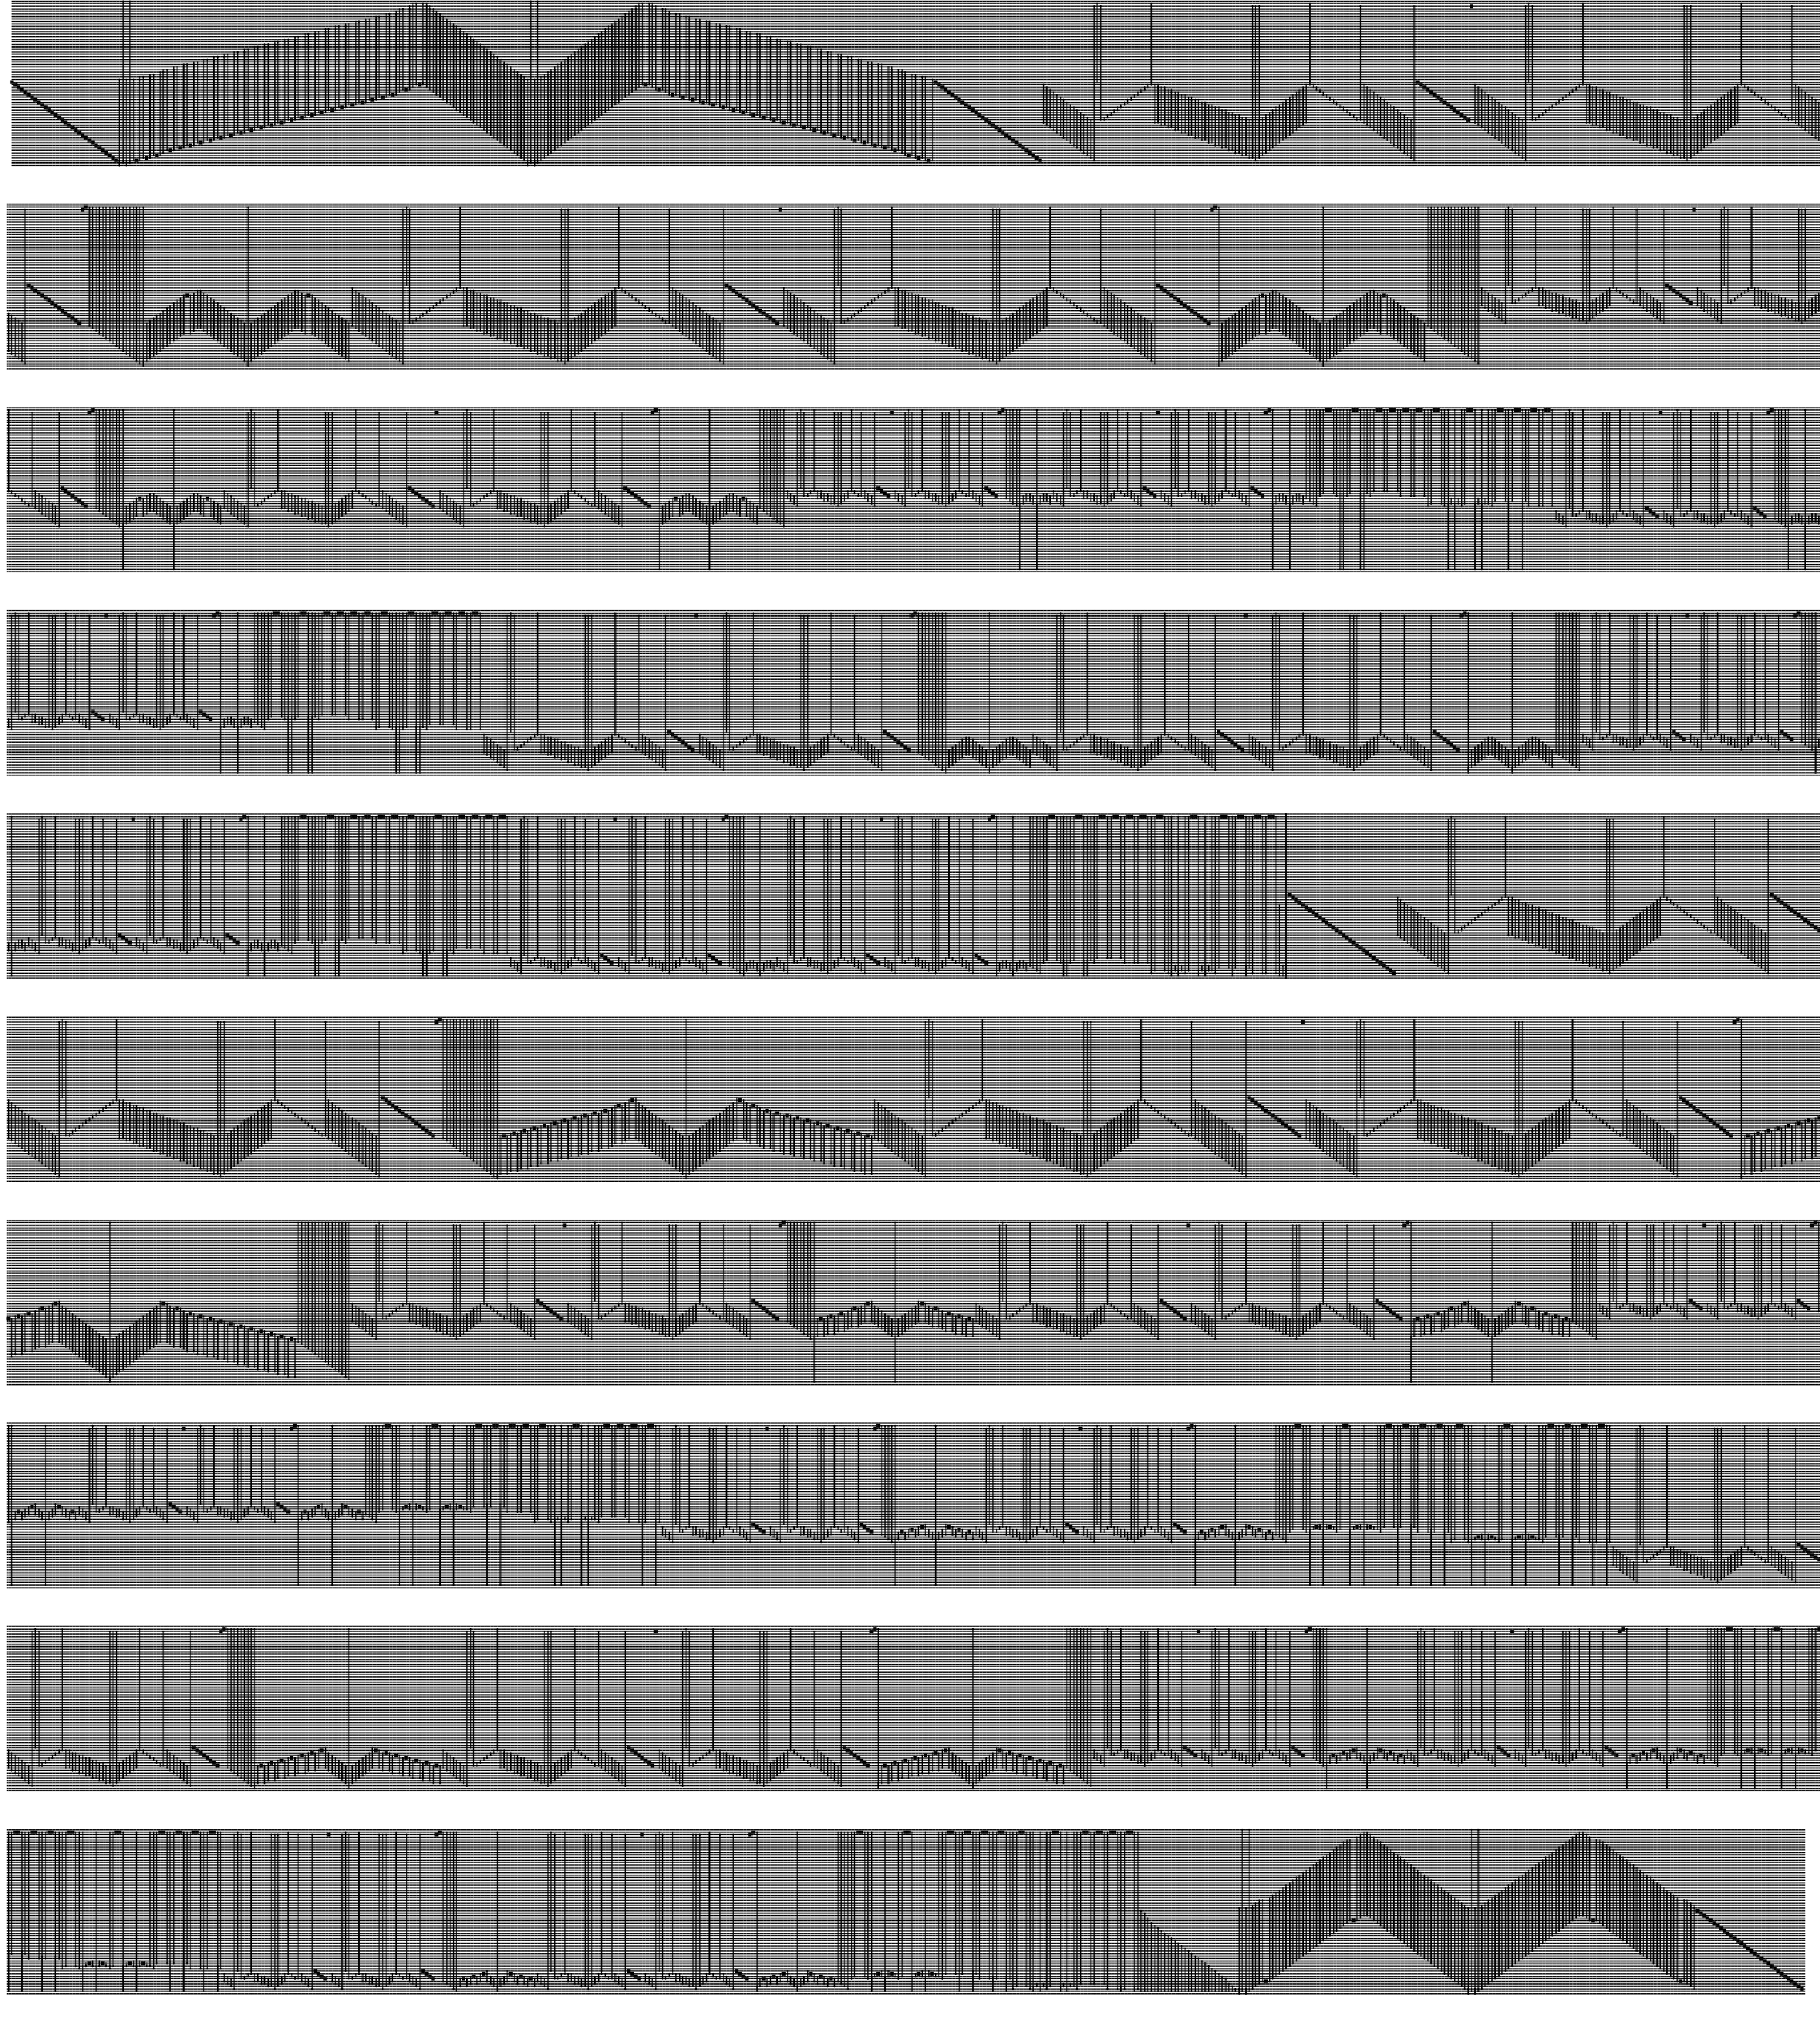
\includegraphics[width=0.9\columnwidth]{pictures/adder.pdf}
\caption{\label{fig:adder} Toffoli network \cite{HRS16} implementing modular inplace addition $x \mapsto x+a$ of the $32$-bit constant $a=4\,294\,967\,291$ to a $32$-bit quantum register. The circuit was rendered in LIQ$Ui|\rangle$, consists of $1813$ Toffoli gates, operates on $32$ qubits and is part of a larger network implementing the controlled modular multiplication needed in Shor's algorithm. The entire modular multiplication $x \mapsto ax\;{\rm mod}\;N$, where $N$ is a $32$-bit modulus, requires $66$ qubits and a total number of $117\,955$ Toffoli gates.}
\end{figure}


\subsection{RUS framework and quantum arithmetic} %the numerical analysis stuff

\begin{figure*}[hbt]
\begin{minipage}{0.45\linewidth}
\[ \Qcircuit @R 1em @C 1.5em { 
\lstick{\ket 0}	&\gate{\phi_1}	&\ctrl{1}		&\gate{-\phi_1}	&\meter\\
		&			&\up{\vdots}  	&				&\\
\lstick{\ket 0}	&\gate{\phi_k}	&\ctrl{1}\qwx	&\gate{-\phi_k}		&\meter\\
		&\qw			&\gate{-iX}	&\qw					&\qw}
\]
%\caption{Gearbox circuit with $k$ inputs\label{fig:GB}, where \\
%the gate $\phi_j$ denotes $e^{-i \phi_j X}$.  Success is \\
%achieved if~{every} measurement reads $0$.}
\end{minipage}
\hspace{0.5cm}
\begin{minipage}{0.45\linewidth}
\[ \Qcircuit @R 1em @C 1.5em { 
\lstick{\ket 0}	&\gate{\phi_1}	&\ctrl{1}		&\multigate{2}{{\rm GHZ}^{-1}}	&\meter\\
		&			&\up{\vdots}  	&				&\\
\lstick{\ket 0}	&\gate{\phi_k}	&\ctrl{1}\qwx	&\ghost{{\rm GHZ}^{-1}}		&\meter\\
		&\qw			&\gate{(i)^{k-1}X}	&\qw					&\qw}
\]
\end{minipage}
\caption{GB (left) and $\rm PAR$ circuit (right) with $k$ inputs\label{fig:PAR}, where 
${\rm GHZ}^{-1}$ is the inverse GHZ measurement.  Success occurs if all measurements read $0$.  PAR implements an approximate multiplication on success and GB an approximate square-multiplier. \label{fig:circuit}}

\end{figure*}

\nix{
\begin{table*}[t!]
\tiny
\[
\begin{tabular}{c@{\qquad}c@{\qquad}c@{\qquad}c}
\hline\\
Circuit & Function & Success probability& Correction circuit\\[1.5ex]
\hline\\
$e^{-i\phi_1 X} e^{-i\phi_2X}$ & $\phi_1+\phi_2$ & $100\%$& --\\[1.5ex]
${\rm PAR}(\phi_1,\ldots,\phi_k)$ & $\prod_{i=1}^k \phi_i + O(\max_i |\phi_i|^{k+2})$&
$\frac{1}{2}\left(\prod_{i=1}^k \cos(\phi_i)^2 + \prod_{i=1}^k \sin(\phi_i)^2\right)$ & $\openone\text{ or } 2{\rm PAR}(\phi_1,\ldots,\phi_k)$\\[1.5ex]
%$\frac{1}{2}(\cos(\phi_1)^2\cdots\cos(\phi_k)^2 + \sin(\phi_1)^2\cdots\sin(\phi_k)^2)$ & $\openone\text{ or } 2{\rm PAR}(\phi_1,\ldots,\phi_k)$\\
${\rm GB}(\phi_1,\ldots,\phi_k)$ & $\prod_{i=1}^k \phi^2_i + O(\max_i |\phi_i|^{2k+2})$&
$\left(1-\prod_{i=1}^k \sin^2(\phi_i)\right)^2 + \prod_{i=1}^k \sin^4(\phi_i)$ &
%$(1-\sin^2(\phi_1)\cdots\sin^2(\phi_k))^2+ \sin^4(\phi_1)\cdots \sin^4(\phi_k)$ 
$e^{-i\pi/4 X}$ (Clifford)\\[1ex]
\hline
\end{tabular}
\]
\caption{Effective transformations carried out by the circuits in \fig{circuit} for small input rotations.\label{tab:succprob}}
\end{table*}
}

It is quite common within quantum algorithms to have transformations
of the form 
%\begin{equation}
$\ket{x}\ket{\psi} \rightarrow \ket{x}e^{if(x)Z}\ket{\psi},$
%\end{equation}
for some function $f$ that maps $\mathbb{B}_{n} \rightarrow \mathbb{R}$.  This form of transformation occurs in algorithms such as the linear systems algorithm~\cite{harrow2009quantum} and also is ubiquitous in quantum machine learning algorithms~\cite{lloyd2016quantum,wiebe2016quantum}.  If we were synthesizing the function $f$  through a reversible circuit we would be in essence approximating $\mathbb{F} \approx \mathbb{F}'$ where $\mathbb{F}' : \mathbb{B}_n \mapsto \mathbb{B}_m$ where $m$ is the number of bits of precision for the output.  Then conditioned on the $m$-bit output the required quantum transformation $e^{i f(x)Z}$ can be synthesized using $m$ controlled single-qubit rotations.  Since these $m$ qubits are only being used in an intermediate step in the algorithm, one can try to avoid them.  

\nix{
Our solution to this problem is inspired in part from the Fourier adder.  The Fourier adder takes advantage of the fact that, for any $(a,b) \in \mathbb{R}^2$
\begin{equation}
e^{ia Z} e^{ib Z} =e^{i(a+b)Z}.\label{eq:phaseadd}
\end{equation}
This shows that if $f(x)$ is a sum then we can use this structure to implement~\eq{target} without requiring any additional ancillae.  However, in order to do this for more general functions we need to have the ability to perform a non-linear operation, such as multiplication.  Since quantum mechanics is a linear theory such non-linear operations a challenge to devise.
}
To achieve this goal, we need to introduce non-linearities.
One approach to generating non-linearities exploits measurement, which is the only non-linear operation in quantum mechanics.  We use two circuits shown in~\fig{circuit} to generate these transformations~\cite{WR16}.  These circuits take its inputs to be the rotation angles that specify a given single-qubit rotation.  They then aim to output a rotation that rotates a qubit through an angle that is approximately the product of the input rotation angles (PAR circuit), or product of their squares (GB circuit).  These circuits achieve this, with high probability, given that their inputs are small.  Furthermore, they can be corrected and the operation can be tried anew if and when they fail.  This ``repeat-until-success'' (RUS) feature is key to their efficiency.

A feature of this approach to constructing an approximate multiplier is that two small numbers can be multiplied in this fashion using only $2$ ancillary qubits independent of the precision of the inputs.  This is because we use an analog degree of freedom, rather than a digital representation, to store the result.  There is, of course, no free lunch.  Higher precision necessitates more error correction, but this only incurrs a logarithmic space overhead and often will be irrelevant given the exacting precision already required of quantum computers by certain algorithms.

Larger numbers can be multiplied using these circuits using ideas from split operator formulas.  In particular, ${\rm PAR}( a,b) = ab + O(\max(a,b)^4)$ and hence for any integer $r>0$,
$r{\rm PAR}(a/\sqrt{r},b/\sqrt{r})=ab + O(\max(a,b)^4/r)$.  Here multiplication by $r$ is implemented by repeating the circuit $r$ times.  Hence by taking $r\rightarrow \infty$ the error can be made arbitrarily small.  Similar tricks, and an algorithm called oblivious amplitude amplification, can be used to make the success probability asymptotically independent of the input rotation angles~\cite{WR16}.

This simple version of the algorithm can be optimized by constructing higher-order multiplication formulas that use GB and PAR to construct a higher-order Taylor series approximation to the product.  As an example ${ab=\rm PAR}(a,b,\frac{\pi}{4}- {\rm GB}(\gamma_2,a)-{\rm GB}(b,\phi_2))+ O(\max(a,b)^6)$ for $\gamma_2 =\arcsin(1/\sqrt{6})$.  We refer to these two lowest order formulas as $M_4$ and $M_6$ respectively.  By iteratively increasing the order of accuracy of the multiplier, $r$ can be made to grow sub-polynomially with the reciprocal of the error tolerance~\cite{WR16}.

We examine the performance of these multipliers in the table below relative to carry-ripple adders and Table-lookup for computing $0.5^2$ at $n=8,16$ bits of precision in the output~\cite{WR16}.
\begin{table}[hbt]
\centering
\footnotesize
\begin{tabular}{c@{\qquad}c@{\quad}c@{\qquad}c@{\quad}c@{\qquad}c@{\quad}c@{\qquad}c@{\quad}c}
\hline
 & \multicolumn{2}{c}{$n=8$\phantom{111}} & \multicolumn{2}{c}{$n=16$} \\[0.2ex]
 {Multiplier}    & $T$-count & qubits & $T$-count & qubits \\
\hline\\
Carry-ripple & 2.80E+03 & 16 & 1.06E+04  &32\\[1.5ex]
Table-lookup  & 3.98E+09 & 2 & 1.13E+13& 2\\[1.5ex]
$M_4$  &4.64E+04 &4 &3.00E+07 &4 \\[1.5ex] 
$M_6$  &3.82E+03 &4 & 5.21E+05&5 \\ 
%$M_8$ & & & & & & & & \\[1ex] 
\hline
\end{tabular}
\end{table}

We see that while the Carry-Ripple multiplier requires more qubits as the precision increases, our multiplier $M_4$ does not.  In fact, the only reason why $M_6$ needs an extra qubit at $n=16$ is because that is the first time where $r>1$ is needed.  This forces us to apply the entire circuit as an RUS-circuit and which requires us to use an additional qubit.  No additional ancillary qubits will be needed as we increase $n$ beyond $16$ for $M_6$.  The number of $T$--gates is intermediate between Table-lookup (which is untenable here) and the Carry-Ripple multiplier.  This demonstrates the space efficiency of our approach and shows that genuinely quantum methods for arithmetic are possible that can reach better tradeoffs between resources than classical strategies can.

As a final note, from the perspective of our synthesis algorithms there is nothing special about multiplication.  We can synthesize any function that is analytic on a compact domain using the Taylor series approach.  Furthermore, this approach can also be used to implement a Chebyshev approximation to a function or even approximate an arbitrary function as a sum of piecewise constant functions~\cite{WR16}.  This flexibility shows that the basic ideas behind this approach are much more general than it may seem at first glance. The ability to compute arbitrary functions in the phase of a qubit provides more than just the first genuinely quantum algorithms for arithmetic: it reveals a new type of ``quantum numerical analysis''.

\section{Conclusion}
As we progress from today's demonstrations of quantum technologies to tomorrows large scale quantum computers, we need to have 
design automation and programming tools in place.  Without such tools, the challenges of designing and testing quantum circuits to implement meaningful
algorithms by hand will be too daunting. 

 Finally, we still need to think broadly about how to approach arithmetic or programming
in quantum computing. While present-day approaches that mimic solutions that have been successful for classical computing provide adequate solutions for now,
it is likely that the solutions of tomorrow may fundamentally differ from anything we can currently imagine.


\bibliographystyle{IEEEtran}
\bibliography{library}

\end{document}

